\makeatletter
\def\input@path{{../}}
\makeatother
\documentclass[../main.tex]{subfiles}

\graphicspath{
	{../img/}
	{../../img/}
	{img/}
}

\begin{document}
\chapter{
	Выпуклая комбинация элементов линейного пространства. 
	Выпуклое множество элементов линейного пространства. 
	Замкнутое полупространство и шар в 
	линейном пространстве 
	$R^n$
	.}

\section{Выпуклая комбинация элементов линейного пространства}
Пусть $p_1, p_2, \dots,p_s$ ~--- точки (вектора), $\alpha_i$ ~---
некоторые числа, такие, что 
$\sum_{i=1}^{s}\alpha_i=1, \alpha_i\geq0 (i=1,2,\dots,s)$.
\textbf{Выпуклой комбинацией} 
точек (векторов) $p_1, p_2, \dots,p_s$ называется точка
\begin{equation}
	p=\sum_{i=1}^{s}\alpha_ip_i.
\end{equation}

\section{Выпуклое множество элементов линейного пространства}
Множество $M$ называется 
\emph{выпуклым}, если для любых двух точек $y$ и $z$ из $M$
справедливо $[y,z] \subseteq M$.
На рис. 1.1a изображено выпуклое множество, 
а на рис. 1.1b  невыпуклое.

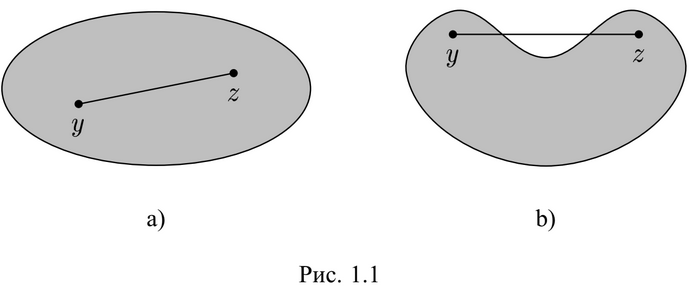
\includegraphics[scale=0.3]{q1_1.png}

Геометрически это означает, что для любых двух точек этого
множества и весь отрезок с концами в этих точках также принадлежит
этому множеству.

\section{Замкнутое полупространство и шар в линейном пространстве 
$R^n$}
Пусть $a = (a_1,a_2,\dots,a_n) \neq 0$. \emph{Замкнутым полупространством} 
называется множество
\begin{equation}
	H(a,a_0)=\{x=(x_1,x_2,\dots,x_n)^T : \sum_{i=1}^{n}a_ix_i \leq a_0\}.
\end{equation} 

\textbf{Утверждение.} \emph{Замкнутое полупространство выпукло}.
\begin{proof}
	Пусть $y = (y_1,y_2,\dots,y_n)^T$ и $y = (y_1,y_2,\dots,y_n)^T$
	~--- две точки замкнутого полупространства $S(a, a_0)$.
	Докажем, что точка $\alpha \cdot z + (1 - \alpha) \cdot y$, 
	где $0 \leq \alpha \leq 1$, также принадлежит
	$S(a, a_0)$. Для этого убедимся в справедливости неравенства
	\begin{equation} 
		\label{question1:1}
		\sum_{i=1}^{n}a_i(\alpha \cdot z_i + (1-\alpha) \cdot y_i) \leq a_0
	\end{equation}
	По определению для точек $y$ и $z$ выполняются неравенства
	\begin{equation}
		\sum_{i=1}^{n}a_iy_i \leq a_0 
		\sum_{i=1}^{n}a_iz_i \leq a_0
	\end{equation}
	Умножая эти неравества соответственно на неотрицательные числа
	$\alpha$ и $(1 - \alpha)$, а затем складывая, получим \ref{question1:1}.
\end{proof}

\emph{Шаром} размерности $n$ радиуса $r$ называется множество
\begin{equation}
	B_n(r)=\{x=(x_1,x_2,\dots,x_n)^T : \sum_{i=1}^{n}x_i^2 \leq r^2\}.
\end{equation}

\textbf{Утверждение.} \emph{Шар является выпуклым множеством}.
\begin{proof}
	Пусть $y = (y_1,y_2,\dots,y_n)^T$ и $z = (z_1,z_2,\dots,z_n)^T$
	~--- точки из $B_n(r)$. Покажем, что точка
	\[ 
		\alpha \cdot z + (1 - \alpha) \cdot = 
		(\alpha z_1 + (1-\alpha)y_1, \dots, \alpha z_n + (1-\alpha)y_n),
	\]
	где $0 \leq \alpha \leq 1$, принадлежит $B_n(r)$. Проделаем
	преобразования:
	\[
		\sum_{i=1}^n(\alpha z_i + (1-\alpha)y_i)^2 = 
		\alpha^2\sum_{i=1}^nz_i^2 + 2\alpha(1-\alpha)\sum_{i=1}^ny_iz_i 
		+ (1-\alpha)^2\sum_{i=1}^ny_i^2
	\]
	Согласно неравенству Коши-Буняковского имеем:
	\[
		\sum_{i=1}^ny_iz_i\leq\sqrt{\sum_{i=1}^ny_i^2} \cdot
		\sqrt{\sum_{i=1}^nz_i^2}
	\]
	Заменяя во всех выражениях 
	$\sum_{i=1}^ny_i^2$ и $\sum_{i=1}^nz_i^2$
	на $r^2$, получаем неравенство
	\[
		\sum_{i=1}^n(\alpha z_i + (1-\alpha)y_i)^2 \leq 
		(\alpha^2 + 2\alpha(1-\alpha)
		+ (1-\alpha)^2)r^2 = r^2,
	\]
	что и требовалось доказать.
\end{proof}
\end{document}